\documentclass[runningheads]{llncs}
%
\usepackage{makeidx}  % allows for indexgeneration
\usepackage[pdftex]{hyperref}
\usepackage{graphicx}
%
\begin{document}
%
\frontmatter          % for the preliminaries
%
\pagestyle{headings}  % switches on printing of running  heads
%
% test line number 2
%
\mainmatter              % start of the contributions
%
\title{
The Electrical Grid and Supercomputer Centers:  
An Investigative Analysis of Emerging Opportunities and Challenges
}

%
\titlerunning{The Electrical Grid and Supercomputing Centers}  % abbreviated title (for running head)
% also used for the TOC unless 
% \toctitle is used
%
%
\author{Fname Lname\inst{1} \and Fname Lname\inst{2}
Fname Lname \and Fname Lname \and Fname Lname \and Fname~M.~Lname \and
Fname Lname}
%
\authorrunning{Fname Lname et al.} % abbreviated author list (for running head)
%
%
\institute{Institute Name, City State Zip, Country,\\
\email{Name@email.adr},\\ WWW home page:
\texttt{http://web/page.html}
\and
Another Institute,
nstitute Department, address1,\\
address2, Country}

\maketitle              % typeset the title of the contribution

\begin{abstract}
Some of the largest supercomputer centers in the United 
States are developing new relationships with their 
electricity providers.  These relationships, similar to other commercial 
and industrial facilities, are driven by mutual interest— to save energy 
costs and improve electricity grid reliability.  Supercomputer centers are concerned about 
electricity price, quality, environmental impact and 
availability. Electricity providers are concerned about 
supercomputer center's impact on the electrical grid reliability, both 
for energy consumption, peak power and fluctuations in 
power. Supercomputer center power demand can be greater 
than 20 megawatts (MW) or more, theoretical peak power requirements 
greater than 45MW and re-occurring intra-hour variability 
can exceed 8MW. As a consequence, there are some 
supercomputer centers whose electricity providers are 
asking for hourly forecasts of power demand, a day in 
advance.   This paper explores today's relationships, 
potential partnerships and possible integration between 
supercomputer centers and their electricity providers and its value. It 
develops a model for possible integration between 
supercomputer centers and the electrical grid. It then 
explores the utility of this model based on feedback from a 
questionnaire of Top 100 List sized supercomputer centers 
in the United States.
\end{abstract}

%
\section{Introduction and Background}
Supercomputer centers with petascale systems for high-performance 
computing (HPC) are realizing the large impact they will be 
putting on their energy service providers with peak power demands of 20MW and instantaneous power fluctuations of 8MW. 
 
The Energy Efficient HPC Working Group 
(\href {http://eehpcwg.lbl.gov/}{EE HPC WG}) 
has been investigating opportunities for large supercomputer sites to more closely 
integrate with their energy service providers. This paper documents the 
results of this investigative activity. 

Leveraging prior work on data center and grid integration opportunities done
by Lawrence Berkeley National Laboratory's (LBNL) Demand Response Research Center
(\href
{http://drrc.lbl.gov/publications/demand-response-and-open-automated-demand-response-opportunities-data-centers}{http://drrc.lbl.gov/publications}),
 this paper takes as a starting point LBNL's model for integrating data
centers and the electrical grid. The model describes programs that are used
by the energy service providers to integrate with their customers (such
as demand response) and methods used to balance the grid supply and demand
of electricity. It also describes strategies that data centers might employ
for managing their electricity and power requirements. This paper tuned this
model's data center strategies for supercomputer centers.  As opposed to data centers, supercomputer centers 
have very high system utilization and are not likely to use virtualization as a strategy.  
Also, supercomputer applications are generally not easily portable between 
geographic locations for a variety of reasons; security, data-locality, system tuning. 
Therefore, although included in the model for data centers, both virtualization and geographic load shifting were eliminated as
potential supercomputer center strategies.


The first section of this paper describes in greater detail the model for
integrating supercomputer centers and the electrical grid. The second
section is a review of prior work on HPC center strategies that might be
deployed for managing electricity and power. In order to further understand
today's relationships, potential partnerships and possible integration
between HPC centers, their energy providers and the grid, a
questionnaire was deployed whose respondents were Top100 List class
supercomputer centers in the United States. The third section of this paper
describes the results of that questionnaire. The fourth section of the paper
describes opportunities, solutions and barriers. A fifth section describes
conclusions and next steps. Finally, the last section recognizes additional
authors.


\label{sec:intro}

\section{Supercomputing Centers and Electrical Grid Integration}
The EE HPC WG Team took as their starting point a model developed by LBNL's 
Demand Response Research Center \footnote{LBNL
Data Center Grid Integration Activities: http://drrc.lbl.gov/projects/dc} that
describes ways in which data centers and electricity service providers may
interact and how this integration can advance new market opportunities. This
integration model describes programs that are used by the electricity service
providers to encourage particular behaviors by their customers and methods used
to balance the grid supply and demand of electricity. It also describes
strategies that data centers might employ for utility programs to manage their
electricity and power requirements and lower costs. The EE HPC WG Team adopted
this model with slight tweaks to reflect the HPC environment (versus the
general data center).

%\href{http://drrc.lbl.gov/publications/demand-response-and-open-automated-demand-response-opportunities-data-centers}
%{http://drrc.lbl.gov/publications}

\subsection{Electricity Demand and Supply Side Management}

Electricity providers use demand-side management for both energy efficiency and to balance the electricity supply. 
Demand side management programs are used to manage the electricity consumption on the consumer’s side of the meter.  
Demand side management can include energy conservation, energy efficiency and peak load management, and responses to 
changing supply conditions.  The focus for this paper is on programs that are targeted at load management. 
Supply side management methods are used to ensure the efficient generation, transmission and distribution of 
electricity.  These methods 
manage the supply of energy on the electricity provider’s side of the meter to meet the changing demand conditions. 

There are many different ways that the end-users of electricity can modify or change their electricity consumption. 
The following is a list and 
brief definitions of key supply-side programs and demand-side management strategies that HPC data centers can utilize:



\begin{itemize}
\item SUPPLY SIDE PROGRAMS
\item Peak Load Response: Programs designed for responses during peak hour “events” and focus on reducing peaks on 
forecasted high-system load days. 
\item Reliability Response: These programs are designed for fastest, shortest duration responses. 
Response is only required during power system and intra-hour variability “events” that typically cannot be forecasted.
\item Regulation Response (Up or Down): Programs designed to follow minute-to-minute commands from the grid to 
balance the aggregate system load and generation. These programs can be expanded to manage the variable and 
uncertain generation nature of many renewable resources, supplement the methods for grid scale storage, which is 
used to store electricity on a large scale to meet the system ramping (up or down) requirements. Pumped-storage 
hydroelectricity is currently one of the largest forms of grid energy storage. Such 
responses can also be used for frequency response, which are methods used to keep grid frequency constant 
and in-balance.
\item Congestion Response: Methods used to resolve congestion that occurs when there is not enough transmission 
capability to support all requests for transmission services.  Or, methods used to resolve congestion 
that occurs when the distribution control system is overloaded. Peak response can be expanded for 
congestion management.
\item Dynamic Pricing: Day-ahead and day-off pricing programs that are designed to change dynamically in response 
to system load and generation conditions.  
\item DEMAND SIDE MANAGEMENT STRATEGIES
\item Load Shed: Strategies used to reduce the load consumption during peak times, 
where the reduced load is not used at a later time.
\item Load Shift:  Strategies where the load during peak times is moved to, typically, non-peak hours.
\item Price Response:  Strategies for time varying and real-time pricing programs used to motivate modification 
to electricity consumption. 
\item Continuous Energy Management: Emerging strategies that modify the load consumption (increase or decrease) 
based on intra-hour changing supply conditions.
\end{itemize}

As the electric grid evolves to a more dynamic and distributed system, its integration with and responses from 
HPC centers can be used to support supply-side programs.

\subsection{Supercomputer Center Response Strategies}

One dimension of the model to response to participate in supply-side programs is a list of demand-side 
management strategies 
that a supercomputer site might use to manage power in response to a request from their electric service provider. 

Although these strategies can be used for managing power in response to a
request from an electric service provider, many of them could also be used
for improving energy efficiency. It is the former that is of primary
interest to this investigation. Two examples may help to clarify this
distinction. Load migration is an example of a strategy that is well suited
to responding to an electric service provider request, but is not likely to
improve energy efficiency. Fine grained power management, on the other hand,
is more likely to be used for improving energy efficiency than for
responding to electric service provider requests.

Below is a list of strategies:

\begin{itemize}
\item Fine grained power management refers to the ability to control HPC system power 
and energy with tools that are high resolution control and can target specific 
low level sub-systems. A typical example is voltage and frequency scaling of the CPU.

\item Coarse grained power management also refers to the ability to control HPC 
system power and energy, but contrasts with fine grained power management in 
that the resolution is low and it is generally done at a more aggregated level. 
A typical example is power capping.

\item Load migration refers to temporarily shifting computing loads from 
an HPC system in one site to a system in another location.

\item Job scheduling refers to the ability to control HPC system power 
by understanding the power profile of applications and queuing the 
applications based on those profiles.

\item Back-up scheduling refers to deferring data storage processes to off-peak periods.

\item Shutdown refers to a graceful shutdown of idle HPC equipment. It usually 
applies when there is redundancy.

\item Lighting control allows for data center lights to be shutdown completely.

\item Thermal management is widening temperature set-point ranges and 
humidity levels for short periods.
\end{itemize}

\label{sec:supercomputing}

\section{Prior Work}
This paper pulls together several diverse research domains. In this section,
we provide an overview of prior work in these areas.

\subsubsection{Power Management}
Processor power management can be divided into two distinct eras. First, with 
the introduction of Dynamic Voltage Frequency Scaling, users were able to 
change the CPU clock speed of their processors, lowering both voltage and,
in most cases, energy: the program used less power and ran longer, but the
quadratic relation of power to frequency biased the results towards overall
energy savings. Early work included several modeling efforts focused on
the effects of CPU- and memory-boundedness on delay and energy in MPI programs~\cite{SpringerPPoPP2006,GeICPP2007,LiHPCA2006,CameronSC2005,HsuSC2005}. 
This work led to the CPUMiser~\cite{GeICPP2007} and Jitter runtime systems, which were designed 
to maximize energy saving consistent with a user-specified delay~\cite{KappiahSC2005}.
Treating energy savings as an optimization problem led to a linear programming
solution~\cite{rountree:07}. The follow-on Adagio runtime system slowed only
computation that could be proven to be off the critical path, leading to significant
energy savings with only negligible slowdown~\cite{rountree:09}. These 
techniques were also applied to non-MPI datacenter workloads~\cite{femal:04}. 

Other power saving approaches were attempted that did not use DVFS, but most
were not deemed relevant to the supercomputing environment. A notable exception
is Dynamic Concurrency Throttling, where energy savings are realized by varying
the number of threads at runtime~\cite{Curtis1,Curtis2,Curtis3}.

The research landscape changed considerably with the introduction of Intel's
Sandy Bridge processor. Turbo mode allowed higher clock frequencies to be
reached so long as fewer cores were in use, making for a nontrivial power- performance tradeoff
calculation. The Running Average Power Limit (RAPL) technology provided an onboard power model that allowed the processor to both
estimate power and, using rapid dithering of CPU clock frequencies, enforce a
user-specified power bound across a short time window~\cite{IntelSDM,David2010}. 
For the first time, users were able to ask questions about performance under 
power bounds. This new capability arrived concurrent with Department of Energy
guideline that exascale machines would be subject to power (as opposed to energy) bounds.

Initial work showed that while processor performance at a fixed frequency 
was reproducible across processors, execution in turbo mode or under a power
bound revealed significant performance variation~\cite{Rountree2012}. Further
work demonstrated a $2x$ performance improvement between conservative and
optimal processor configurations while executing under a power bound~\cite{Patki1}.

\subsubsection{Thermal Management}

Thermal management is a key driver for improving energy efficiency of datacenters as well as SCs. There are many strategies for thermal
management that can improve energy efficiency, such as free cooling and proper
airflow. This paper discusses two thermal management strategies that have an
opportunity for grid integration. The first strategy is controlling the inlet
temperature to the computing equipment, raising it as high as possible without
causing reliability induced hardware failures. The second strategy is using
thermally aware job scheduling.

In 2011, the American Society of Heating, Refrigeration and Air Conditioning
(ASHRAE) datacenter Technical Committee TC9.9 published guidelines that
expanded the environmental range for datacenters and SCs~\cite{ASHRAE:tgfdpe}. The environmental range includes factors such as temperature, humidity
and dew point and allowable rate of change. This expansion allows for
maintaining high reliability while achieving gains in energy efficiency. These
guidelines continue to be updated and the range continues to expand as the
industry collects more historical data showing trade-offs between reliability
and environmental factors.

It is implicit in the ASHRAE guidelines that a SC might be
able to increase temperature as a response to a request from an ESP. The guideline defines both recommended and
allowable environmental ranges. It also specifies a maximum rate of
change, which is most stringent for tape drives. For SCs, the
difference between the maximum recommended and allowable dry bulb temperature is
a minimum of 9 degrees F. The rate of change for tape drives is 9 degrees F per
hour (36 degrees F for solid state computing systems). Therefore, assuming
that SCs normally operate within the recommended range and
that they are willing to operate on occasion in the allowable range (or beyond),
it is theoretically possible to stay within ASHRAE thermal guidelines and use
temperature excursion as a grid-integration strategy. 

ASHRAE has also published a guideline on liquid cooling environmental ranges. At this point, however, the guidelines do not document rate of
change for liquid temperature. Although it is not explored in this paper, it
may be possible to use increases in liquid cooling temperature as a
grid-integration strategy as well. 

Ghatikar et. al \cite{Ghatikar2012a} describe field studies on using thermal
management as a grid-integration strategy. They demonstrate increasing ``facility HVAC temperature set points in order to decrease HVAC power
demand” in two different field locations. There was only a small
electricity demand decrease demonstrated.

Runtime cooling strategies are mostly job-placement-centric. These techniques
either aim to place incoming computationally intensive jobs in a thermal-aware
manner on servers with lower temperatures or attempt to migrate or load-balance
jobs from high-temperature servers to servers with lower temperatures.

Kaushik et. al \cite{kaushik_t*:_2012} proposed \emph{T*}, a system that is
aware of server thermal profiles and reliability as well as data semantics
(computation job rates, job sizes, etc). This system saves cooling energy costs
by using thermal-aware job placements without trading off performance.

Sarood et. al \cite{SaroodSC11} designed a runtime system that does
temperature-aware load balancing in datacenters using DVFS and task migration.
They also discussed how hotspots could be avoided in datacenters, and showed
cooling costs can be reduced by up to 48\% with temperature-aware load
balancing.

\subsubsection{Job Scheduling}
The problem of scheduling jobs has been extensively studied. Most resource
managers implement the First Come First Serve (FCFS) policy as a simple but fair
strategy for scheduling jobs. However, FCFS suffers from low system utilization.
A common optimization is \emph{backfilling}~\cite{lifka_anl/ibm_1995,mualem_utilization_2001,feitelson_parallel_2004}.
Backfilling improves system utilization by executing jobs with small resource
requests out of order on idle nodes.

Fan et al. \cite{PowerAwareServer1} discussed power-aware job scheduling in the
datacenter domain. They discussed a power monitoring system that could use
power capping (based on a power estimation method such as RAPL or direct power
sensing) and a power throttling mechanism. Such as system works well when is a
set of jobs with loose service level guarantees or low priority that can be
forced to reduce consumption when the datacenter is approaching the power cap
value. Etinski et al. \cite{Etinski1,Etinski2,Etinski3,Etinski4} explored
scheduling under a power budget in supercomputing and analyzed bounded slowdown
of jobs. In their series of papers, they introduced three policies. Their first
policy is based looks at current system utilization and uses DVFS during job
launch time to meet a power bound. Their second policy meets a bounded slowdown
condition without exceeding a job-level power budget. Their third policy
improves upon the former by analyzing job wait times and adding a reservation
condition. 

There are many use cases in a grid computing environment that require QoS
guarantees in terms of guaranteed response time, including time-critical tasks
that must meet a deadline. Foster et. al~\cite{foster_distributed_1999,foster_anatomy_2001} proposed \emph{advance
reservations} to achieve time guarantees. Advance reservation is a guarantee for
the availability of a certain amount of resources to users and applications at
specific times in the future. The advance reservation feature requires
scheduling systems to support reservation capabilities in addition to
backfilling-based batch scheduling. Modern resource management systems such as
Sun Grid Engine, PBS, OpenPBS, Torque, SLURM, Maui, and Moab support advance
reservation capabilities.

\subsubsection{Load Migration}
Chiu et. al \cite{chiu_electric_2012} discussed a electrical grid balancing
problem that was experienced in the Pacific Northwest. In order to match
electricity supply and balance the electrical grid, they proposed low-cost
geographic load migration. They also suggested that a symbiotic relationship
between datacenters and electrical grid operators that leads to mutual cost
benefits could work well. Ganti et al. \cite{Ghatikar2012b} looked at two
applied cases for distributed datacenters. The results show that load migration
is possible in both homogenous and heterogeneous systems. Their migration
strategies were based on a manual process and can benefit from automation.

\subsubsection{Dynamic Pricing}
Aikema et. al \cite{aikema_electrical_2011} explored the potential for HPC
centers to adapt to dynamic electrical prices, to variation in carbon intensity
within an electrical grid, and to availability of local renewables. Their
simulations demonstrated that 10- 50\% of electricity costs could potentially
be saved. They also concluded that adapting to the variation in the electrical
grid carbon intensity was difficult, and that adapting to local renewables could
result in significantly higher cost savings.

Power-aware resource management without degrading utilization has been proposed
as a DR strategy to reduce electricity costs
\cite{yang_integrating_2013,zhou_reducing_2013}. The novelty of the proposed job
scheduling mechanism is its ability to take the variation in electricity price
(dynamic pricing) into consideration as a means to make better decisions about
job start times. Experiments on an IBM Blue Gene/P and a cluster system as well
as a case study on Argonne's 48-rack IBM Blue Gene/Q system have demonstrated
the effectiveness of this scheduling approach. Preliminary results show a 23\%
reduction in the cost of electricity for HPC systems.
\label{sec:priorwork}

\section{Questionnaire} 
We used a questionnaire in order to understand the current experiences of
supercomputer centers with respect to interacting with their electricity
service providers. We restricted the analysis to sites in the United States
since the results of the survey and practices of demand response is highly
correlated and driven by energy policies in the country. 
\cite{torriti_demand_2010}
[Tor10].

Nineteen Top100 List sized sites in the United States were targeted for the
questionnaire. Eleven sites responded (Oak Ridge National Laboratory, 
Lawrence Livermore National Laboratory, 
Argonne National Laboratory, 
Los Alamos National Laboratory, LBNL, 
Wright Patterson Air Force Base,
National Oceanic Atmospheric Administration, 
National Center for Supercomputing Applications, 
San Diego Supercomputing Center, 
Purdue University and Intel Corporation). Eight sites didn't respond (
National Center for Atmospheric Research,
IBM Corporation, 
National Energy Technology Laboratory, Indiana University, 
Texas Advanced Computing Center, 
Sandia Natinal Laboratory, 
National Renewable Energy Laboratory, 
National Aeronautics and Space Administration). The questionnaire was
sent to a sample that was not randomly selected. It was sent to those sites
where it was relatively easy to identify an individual based on membership
within the EE HPC WG. The sample is more representative of Top50 sized sites
(1 Top50 sized site was not in the sample and 60{\%} (9/15) of the sample
responded). Only 4 additional sites were sampled from the Top51-Top100 List
and, of those, 2 responded (Intel and National Oceanic and Atmospheric Administration).

The total power load as well as the intra-hour fluctuation of these sites
varied significantly. There were four sites with total power load greater
than 10MW, two sites with \textasciitilde 5MW total power load and five
sites with less than 2MW total power load. We chose less than 3MW intra hour
variability as the bottom of the scale because we assumed that the
electrical service providers would not be affected by that magnitude of
fluctuation. For those with total power load greater than 10MW, the
intra-hour fluctuation varied from less than 3MW to 8MW. One of
\textasciitilde 5MW sites said that they experienced 4MW variability. The
rest of the sites were all less than 3MW. Most of the intra-hour variability
was due to preventative maintenance.


\begin{table}[htbp]

\begin{center}
\caption{Caption Number 1}
\begin{tabular}{|p{65pt}|l|l|}
\hline
\textbf{Total Load}&
\textbf{Variability}&
\textbf{Frequency} \\
\hline
16-17MW&
5MW&
weekly \\
\hline
13-14MW&
8MW&
monthly \\
\hline
10-11MW&
Less than 3MW&
weekly \\
\hline
10-11MW&
7MW&
weekly \\
\hline
4-5MW&
Less than 3MW&
weekly \\
\hline
4-5MW&
4MW&
weekly \\
\hline
1-2MW&
Less than 3MW&
weekly \\
\hline
1-2MW&
140kW&
daily \\
\hline
1-2MW&
Less than 3MW&
yearly \\
\hline
1-2MW&
200kW or less&
daily \\
\hline
1-2MW&
Less than 3MW&
daily \\
\hline
\end{tabular}
\label{tab1}
\end{center}
\end{table}

We asked if the supercomputer centers had talked to their electric service
providers about programs and methods used to balance the grid supply and
demand of electricity. About half of them have had some discussion, but it
has mostly been limited to demand side and not supply-side programs.


\begin{table}[htbp]

\begin{center}
\caption{Caption Number 2}
\begin{tabular}{|p{230pt}|l|}
\hline
\textbf{Discussions with Electricity Providers}&
{\%} Answered Yes \\
\hline
\textbf{Programs}&
~ \\
\hline
Shedding load during peak demand&
54 \\
\hline
Responding to pricing incentive programs&
45 \\
\hline
Shifting load during peak demand&
36 \\
\hline
\textbf{Methods}&
~ \\
\hline
Enabling use of renewables&
36 \\
\hline
Congestion, Regulation, Frequency Response&
18 \\
\hline
Contributing to electrical grid storage&
10 \\
\hline
\end{tabular}
\label{tab2}
\end{center}
\end{table}

More than half of the respondents are not interested in shedding or shifting
load during peak demand. There is some indication that this low interest is
primarily due to the lack of a clear business case. For the sites where
there is interest, shifting is more attractive than shedding load. The San Diego Supercomputing Center (SDSC) is
an exception to this trend, but because of a site-wide program. ``University of California San Diego
generates 30-35MW of power yet still imports 5-10MW. As a large generation
source the utility providers see the campus as a highly attractive partner
for offloading grid stress. Automatic load shedding is being
explored/deployed today.''

Responding to pricing incentive programs is also not considered interesting,
although the reasons for this low interest may be organizational. Several
open-ended comments revealed that pricing is fixed and/or done by another
organization at the site level and outside of their immediate control.

Eighty percent of the respondents have not had discussions with their
electricity service providers about congestion, regulation and frequency
response. Los Alamos National Laboratory (LANL) is one of two who have had discussions and who commented that
they are ``learning about the process'' and that it is ``outside of [their]

visibility or control''.

There were been many more respondents who have had discussions with their
electricity service providers about enabling the use of renewables; 36{\%}
have already had discussions and more than half are interested in further
and/or future discussions. SDSC already has a site-wide program; ``the
campus has a large fuel cell (2.5$+$ MW) and works with the utility with
renewables.'' Other responses suggest that the interest is at the site level
and not unique to the supercomputer center.

An open-ended question was posed as to whether or not there was information
either requested of the supercomputer sites by their providers or,
conversely, requested of the providers by the sites. In both cases, well
over 75{\%} of the respondents answered no. Lawrence Livermore National Laboratory (LLNL) and LANL were the
exceptions. LLNL is ``working on obtaining additional data from them and a
means of sharing data between them and us'' and has been requested to
provide ``additional detailed forecasting and ultimately real time data.''
LANL has also been requested to provide ``power projections, hour by hour,
for at least a day in advance'' and, perhaps as a consequence, would like to
have more information on ``sensitivity of power distribution grid to rapid
transients (random daily step changes of 10 MW up or down within a single AC
cycle).''

Given the low levels of current engagement between the electricity service
providers and the supercomputer centers, it is not surprising that none of
the supercomputer centers are currently using any power management
strategies to respond to grid requests by their electrical service
providers. SDSC's \textit{supercomputer center} is not an exception, but they did respond that their
entire ``campus is leveraging parallel electrical distribution to trigger
diesel generators and other back-up resources to respond to to grid and
non-grid requests.''

We tried to evaluate if power management strategies will be considered
relevant and effective for grid integration at some point in the future. Two
questions were asked; is there interest in using the strategies and what
impact did they think that the strategies would have. When combining
interest and impact, the results showed that power capping, shutdown, and
job scheduling were both high interest and impact. Load migration, back-up
scheduling, fine grained power management and thermal management were medium
interest and impact. Lighting control and back-up resources were low
interest and impact.


\begin{table}[htbp]

\begin{center}
\caption{Caption Number 3}
\begin{tabular}{|p{299pt}|}
\hline
\textbf{HPC strategies for responding to Electricity Provider requests (listed from highest to lowest interest }$+$\textbf{ impact)} \\
\hline
Course grained power management \\
\hline
Facility shutdown \\
\hline
Job scheduling \\
\hline
Load migration \\
\hline
Re-scheduling back-ups \\
\hline
Fine grained power management \\
\hline
Temperature control beyond ASHRAE limits \\
\hline
Turn off lighting \\
\hline
Use back-up resources (e.g., generators) \\
\hline
\end{tabular}
\label{tab3}
\end{center}
\end{table}

\label{sec:questionaire}

\section{Opportunities/Solutions and Barriers} 
The responses to the questionnaire presented in
Section~\ref{sec:questionnaire} represent a variety of desires and
experience regarding interactions between supercomputer centers and
electricity service providers.  For example, the responses from the two centers
with the largest power draws, Lawrence Livermore National Laboratory
(LLNL) and Oak Ridge National Laboratory (ORNL), diverge in several
areas.  This divergence is perhaps primarily due to characteristics of
their respective electricity service providers.  In contrast, San Diego
Supercomputer Center (SDSC) stands out as a leader in integrating
with their electricity service provider on a site-wide level.  To that end, the
responses from SDSC may exemplify some of the opportunities available
to other supercomputer centers that are willing to pursue this degree
of integration.

% The following paragraph is what we want to claim, but is actually
% factually incorrect.  A supercomputer center understands its
% cost to operate per unit time (e.g., cost to run per hour).  This
% cost includes things like the cost of personnel, cost of renting
% the physical space for the supercomputer center, cost of electricity, etc.
% It turns out that the cost of electricity is a small percent of
% the overall cost of running the center.  In the end, I think there
% is very little chance of getting supercomputer centers to
% willingly negotiate with electricity service providers because the cost of
% the lost opportunity is too high since the remaining costs are
% unchanged.
The responses to the questionnaire also suggest that some electricity service
providers are requesting that their supercomputer center customers
develop capabilities for informing the provider of expected periods of
exceptional power consumption and for responding to requests from the
provider to consume less power for specified periods of time.  Upon
initial consideration, this idea might seem to run counter to the
primary mission objective of most supercomputer centers of delivering
as many uninterrupted computational cycles as possible to their users.
In some extreme cases, supercomputer centers may not have a choice
in the matter as the size and energy requirements of supercomputers
increase; indeed, some electricity service providers may \textit{require} large
centers to develop a demand-response capability.  However, a direct
business case may exist to encourage supercomputer centers to develop
this negotiation capability on their own.  For example, if electricity service
providers were to offer electricity at a significantly reduced rate
on the condition that the supercomputer center customer develop
demand-response capabilities, the long-term cost savings to the
center could make undertaking such a project worthwhile.

Perhaps one of the most straightforward ways that supercomputer
centers can begin the process of developing a demand-response
capability is by enhancing existing system software used for managing
computing resources within the center.  Indeed, the questionnaire
responses from Section~\ref{sec:questionnaire} as well as the literature
review presented in Section~\ref{sec:priorwork} both strongly support the
idea that the greatest opportunities for supercomputer centers to
develop integration capabilities are related to system software.
Specifically, and presented in approximate order of decreasing
interest and expected impact to the questionnaire respondents, system
software in this context consists of coarse-grained power management
in the form of power capping, job scheduling, load migration,
rescheduling backups, and fine-grained power management.

Coarse-grained power capping may be one of the most straightforward
methods of power management.  In the simplest form, this technique may
entail human intervention to adjust computing resources so they
operate at a reduced capacity or to entirely shut down some of the
computing capacity of a supercomputer center.  By attenuating
resources, the supercomputer center manager can ensure that power
consumption stays below some defined level.  This defined level may be
a pre-arranged power cap negotiated between the supercomputer center
and the electricity service provider and maintained on an ongoing basis,
or, perhaps more likely, a power draw level that is requested by the
electricity service provider to handle unanticipated loads somewhere else
in the electricity service provider's system.  One important thing to
notice in using this approach to power management is that the savings
in power may not need to come entirely from attenuating computing
resources.  Rather, reducing power consumption in computing resources
is likely to result in a corresponding reduction in thermal load
within the supercomputer center.  This reduction in thermal load
may allow a significant degree of power saving to occur by requiring
less power to be spent on air conditioning.

The coarse-grained power capping technique described above assumes
that the supercomputer center environment has some amount of
instrumentation and metering that allows for the collection of power
telemetry data.  This telemetry is necessary for the supercomputer
center facility manager in order to understand how the power supplied
by the electricity service provider is distributed to resources within the
center.  Further, this telemetry is likely important to automated
solutions for power management, such as the job scheduling techniques
described below.  In light of the fact that many system integrators
such as Cray and IBM are now delivering supercomputer systems that
include telemetry capabilities, the assumption that this information
is available seems acceptable.  According to the responses to the
questionnaire presented in the previous Section, supercomputer center
facility managers perceive this accounting data as distinct from
per-user or per-job accounting data that is typically collected and
indicate that this data should be retained for electricity
provisioning planning purposes.

Techniques that involve job scheduling may offer more automated
approaches to power management.  Due to the unique role that the job
scheduler and resource manager play within a supercomputer center,
these techniques may involve adjusting either the workflow of jobs
within the center or characteristics of the computational resources
within the center.

% I (koenig) would be able to self-cite out of my own publications
% concepts such as ``priority'' and ``urgency'' described in the
% following paragraph.  If desired, we would need to add these
% papers into the bibliography and/or related works section.
On one hand, the job scheduler has knowledge of and control over the
upcoming workflow within the supercomputer center simply by examining
and manipulating the job queue.  One easily-accessible technique is
for a human operator to use capabilities such as advanced reservations
to reserve pre-arranged blocks of time in which jobs with high power
loads will run.  These blocks of time could be negotiated with the
electricity service provider on an ongoing basis or could be in response to
on-demand requests made by the electricity service provider.  Even more
automatic techniques are possible if the job scheduler is given enough
information about the workflow to make intelligent decisions about job
scheduling.  For example, jobs may be submitted with various metadata
that enable the job scheduler to understand characteristics of each
job such as \textit{priority}, the relative importance of a job
compared to other jobs, and \textit{urgency}, the rate at which the
value of a job decreases as time elapses.  These characteristics are
not only important to a job scheduler for ensuring efficient
utilization of a supercomputer center's resources under traditional
circumstances, but they are also a vital piece of successfully
implementing a demand-response capability for at least two reasons.
First, they provide a set of metrics by which the supercomputer center
can estimate the cost in terms of the ``lost opportunity'' of
responding to an electricity service provider's request to run with
attenuated resources.  Second, they allow the supercomputer center to
prioritize jobs in the queued workflow in order to understand how to
best utilize computational resources.  This capability is important
under normal circumstances, but becomes even more essential in a
demand-response scenario.

On the other hand, the job scheduler has knowledge of and control over
the computational resources within the supercomputer center, giving
the job scheduler several mechanisms for implementing a
demand-response capability.  Most of these mechanisms could be
considered fine-grained power control mechanisms because they mostly
tune low-level settings on the nodes and processors within the
supercomputer center.  For example, the job scheduler knows which
nodes within a supercomputer are occupied with running jobs or are
expected to become occupied in the near future.  To that end, the job
scheduler can use its control over the resource management process to
place idle nodes into a sleep state in which they draw significantly
reduced power.  This strategy is especially effective in supercomputer
environments containing at least some resources that are used at
irregular intervals, allowing opportunities to utilize sleep states
effectively during periods when the resources are idle.  In
environments where all computing resources are heavily utilized most
of the time, more sophisticated strategies that require the job
scheduler to rely on knowledge about each batch job may be necessary.
Such knowledge might come from the type of metadata described in the
previous paragraph or from a database that is maintained based on
previous runs of jobs submitted by each user.  For example, if the job
scheduler knows that a given job contains mostly I/O operations, or
consists of discrete phases where I/O occurs, the job scheduler might
choose to adjust the Performance State (P-state) for each processor
running the job in a way that reduces the job's overall power
consumption.  The P-state mechanism is a way of scalably adjusting a
CPU's frequency and voltage operating points which in turn causes the
processor to consume less power directly and to produce less thermal
load indirectly.  In cases where a processor is executing a
processing-intense task, gating the processor's P-state often has a
noticeable impact on the overall task performance; however, in cases
where a processor is executing a mostly I/O-bound task, gating the
processor's P-state typically does not make a noticeable impact on the
overall task performance due to the fact that the processor spends a
great deal of time blocked waiting for I/O operations to complete.

Even more interesting scenarios are possible in cases where the job
scheduler combines its knowledge of the upcoming queued workflow with
its knowledge and control over the computational resources within the
supercomputer center.  These scenarios are most appropriate when the
supercomputer scenario contains a pervasively heterogeneous mix of
computational resources.  For example, many contemporary supercomputer
centers contain several different types of compute nodes with various
types of processors and accelerator cards.  In some circumstances, the
job scheduler may be able to choose which resource to use for running
a given job among several candidate resources.  The trade-off here is
not only in terms of the time necessary to complete the job (i.e.,
different resources could potentially complete the job in very
different amounts of time) but also in terms of the energy consumed in
completing the job (i.e., different resources could potentially
consume very different amounts of energy in completing the job).
Further, other resources such as memory access patterns, disk access
patterns, and network use affect the energy signature of a job and may
be observed by the scheduler.  By maintaining a database of
job-to-resource mappings that record the time and energy taken for
each job, the scheduler can, over time, improve its ability to decide
which jobs have the highest affinity to each type of resource.  Using
this knowledge to optimize a supercomputer center's workflow in terms
of job throughput or energy consumption is admittedly complex, but the
potential rewards are likely to be compelling both to the day-to-day
operation of the center and to demand-response capabilities.

Opportunities may also exist for supercomputer centers to cooperate
with each other in scenarios in which computational loads are migrated
from one site to another where energy costs are less expensive.  This
scenario is challenging for both technical and business reasons.
Technical challenges include issues such as user authentication and
authorization (i.e., a user may be authorized to use resources at one
site but not at another site) and data movement (i.e., it may be
infeasible to migrate large datasets from one site to another site).
To some extent, some of these technical challenges may be mitigated by
the use of advanced reservation capabilities in the scheduling systems
at each site, allowing resources to be simultaneously reserved while
large datasets are properly staged.  Business challenges include the
notion that a supercomputer center currently has little incentive to
migrate jobs to another ``competing'' center.  Indeed, the
questionnaire results reflect low interest in load migration
strategies.  It seems likely that in order to be a feasible scenario,
the structure of payment and rewards to a supercomputer center to
cooperate with other centers would need to be structured differently
than they are currently.

In a very broad sense, demand-response techniques such as job
scheduling, power capping, and load migration can be considered to
be coarse-grained approaches because they involve considering ``big
picture'' views of the workload and computational resources in a
supercomputer center.  According to the questionnaire results
presented in the previous Section, facilities managers view these
approaches as the most likely candidates for creating effective
demand-response capabilities.

Finally, this Section has focused heavily on the opportunities
available to supercomputer centers that come from developing
demand-response capabilities.  This notion is primarily due to the
fact that the questionnaire presented in Section~\ref{sec:questionnaire}
was distributed to supercomputer centers in the United States, not to
electricity service providers.  That said, opportunities do exist for
electricity service providers that develop demand-response
capabilities.  At one level, the negotiation process itself requires
integration in terms of the communication and messaging protocols that
are necessary.  To that end, opportunities exist for adapting and
extending existing standards currently used within the industry, thus
creating new use cases and capabilities for electricity service
providers.  At a higher level, electricity service providers will most
likely need to improve their ability to determine in near real time
the important places within the electrical grid where demands exceed
supply.  Determining this is likely to be a complex optimization
problem.  While this Section focuses on solving these problems to the
end of developing a demand-response strategy in conjunction with
supercomputer centers, these capabilities are likely applicable to a
broad range of customers.

\label{sec:opportunities}

\section{Conclusions and Next Steps}
%This section is a work in progress
%
\begin{enumerate}
\item Potential HPC-specific value proposition for active DR engagement
\item Based on Grid Integration solutions -- local and system-wide impacts
\item Next steps -- specific directions or target areas to focus
\end{enumerate}

In past, electricity providers have viewed the hourly, daily, and seasonal
fluctuations of demand as facts of life. These fluctuations required
additional generating capacity, particularly peaking plants that were needed
only a few hours per year. 

However, with increasing adoption of Smart Grid, information technology, communications, and a more dynamic and reslient grid, 
the value proposition of replacing the expensive and fossil-based peaking plants with more predictable demand with forecasting and demand response has the potential for new value proposition to the HPC data centers. 
The increase in renewable generation and its intermittency offers opportunities for large and flexible loads that can adapt to changing electricity generation and sources.

DR adoption: 
Automation: 
%
As the previous research as shown with data centers, HPC can also be considered as a resource to the grid and provide different services.
To enable this, automation technologies, which can link the HPC data centers with the electric grid, 
and on-site power management strategies for different timescales for grid services will play a key role in ease of adoption and lowering the participation costs.

Electriicty markets: 
One of the key enabler for HPC data centers to participate in electriicty markets (e.g., demand response, electricity prices)
is the markets that value their participation. 
In other areas of commercial buildings and select industrial facilities, benefits to both electricity service providers and customers are well documented.
However, as the electric grid and new dynamic loads such as HPCs evlove, the markets need mechanisms to identify and provide value of participation (e.g., cost, energy, carbon). 
(LIST SOME KEY FINDINGS FROM QUESTIONNAIRE)

value proposition, (INCLUDED IN THE ELECTRICITY MARKETS ABOVE)

the measurement and verification models, (LISTED BELOW)

patents, (NOT SURE WHAT THIS IS AND WHY THIS IS RELEVANT)

intellectual property (NOT SURE WHAT THIS IS AND WHY THIS IS RELEVANT)

lighting, and heating, ventilation, and air conditioning (HVAC)
It is clear from the HPC operation that the largest opportunity for load management exists in the IT equipment.
However, the previous work suggests that the opportunity in HVAC loads may also be an immediate opportunity. 
The opportunity depends on the ratio of cooling loads to the IT equipment load (e.g., PUE).
Considering that the lighting loads are a small percentage of overall HPC load, their participation alongside other strategies (IT equipment and HVAC) may prove beneficial. 
The advancement in technologies and vendor recognition to provide more dynamic power management capabilities in the IT equipment offers larger opportunity in consolidated IT and cooling load reductions.

electricity-price markets (INCLUDED IN THE ELECTRICITY MARKETS ABOVE)

interoperability

The grid integration need to be standardized and provide interoperable
interfaces to be interoperable. Interfaces, communication infrastructure,
data, information exchange, agreement should be based on standards.
Communication with grid providers need to be standardized. grid
request/response messages. Requests include DR event, price, renewable
generation


How is architected an accounting system (energy and utilization) of an HPC
center? based on sensor systems like in [Hay09] . Sensor systems for an HPC
center to report real time power consumption of various components such as
cooling, compute systems, storage, networks, racks, etc.

[Hay09] S. Hay and A. Rice, ``The case for apportionment,'' in Proceedings
of the First ACM Workshop on Embedded Sensing Systems for Energy-Efficiency
in Buildings, New York, NY, USA, 2009, pp. 13--18.

Apportioning the total energy consumption of a building or organization to
individual users may provide incentives to make reductions. We explore how
sensor systems installed in many buildings today can be used to apportion
energy consumption between users. We investigate the differences between a
number of possible policies to evaluate the case for apportionment based on
energy and usage data collected over the course of a year. We also study the
additional possibilities offered by more fine-grained data with reference to
case studies for specific shared resources, and discuss the potential and
challenges for future sensor systems in this area.

\begin{itemize}
\item If accounting data can be used to forecast and model future energy usage of an HPC center? so this can be communicated and be in
integrated with electricity grid.
\item If/how electricity grid providers can use energy and usage accounting data to plan electricity provisioning of an HPC center?
\item user-specific accounting data versus workload-specific accounting data.
\item accounting data in terms of HPC center components, cooling, systems, lighting, etc.
\end{itemize}
These are excellent questions. What you've outlined below is a set of value
of real-time data (the term "accounting" confused me earlier) of energy and
utilization for HPC systems. Some of these values are for EE and the rest is
how the electric grid service providers can benefit from it. For example,
telemetry data for wholesale DR markets and M{\&}V.

M{\&}V or Measurement and Verification refers to quantification of load shed
that a particular load is participating in. Typically, there are many
baseline methodologies that the utilities and ISOs use to calculate the
amount of DR a particular load/facility is providing through real-time and
day-ahead metered data. The metering and telemetry to provide the M{\&}V is
key in determining if a particular resource can participate in a DR market 
and validate its performance for settlement (economics).


\label{sec:conclusion}

\newpage


%
% ---- Bibliography ----
%
\bibliographystyle{abbrv}
\bibliography{../bib/whitepaper}  % eehpcmethod.bib is the name of the Bibliography in this case
%

\section{Appendices}

\subsection{Background}

Over the last few years, load growth, increases in intermittent generation,
declining technology costs and increasing recognition of the importance of
customer behavior in energy markets have brought about a change in the
focus of DR in Europe [Tor10]. The long standing programs involving large
industries, through interruptible tariffs and time of day pricing, have been
increasingly complemented by programs aimed at commercial and residential
customer groups.

\cite{torriti_demand_2010} Tor10] examines experiences within European countries as well as at
European Union (EU) level. While business programs, technical and economic
potentials vary across Europe, there are common reasons as to why
coordinated DR policies have been slow to emerge: the limited knowledge on
DR energy saving capacities; high cost estimates for DR technologies and
infrastructures; and policies focused on creating the conditions for
liberalizing the EU energy markets.


advances in DR It describes initiatives, studies and policies of various
European countries, with in-depth case studies of the UK, Italy and Spain.

Spees, K., {\&} Lave, L. B. (2007). Demand Response and Electricity Market
Efficiency. \textit{The Electricity Journal}, \textit{20}(3), 69--85. doi:10.1016/j.tej.2007.01.006

Interruptible Programs represent 6.5{\%} of peak power and Load Shedding
Programs initiate automatic load shedding in emergency situations [30].
With Interruptible Programs participants are required to reduce their load
to predefined values. With Load Shedding Programs utilities have the
possibility to remotely shutdown participants' equipment at short notice.
One significant difference between these two programs is that for
Interruptible Programs participants who do not respond can face penalties.


Load Shedding Programs are divided into real time programs (without
notice) and 15 min notice programs. The size ranges from 1200 MW for real
time programs to 1750 MW for notice programs. Participants in these
programs have to install and maintain Load Shedding Peripheral Units and
will be compensated according to a non-market price defined in regulation.
The size of curtailable power is of 10 MW for programs without notice and
3 MW for programs with notice.

Load forecasting is very important for power system operation and planning.
Traditional load forecasting tools have limitations to reflect DR customer
behaviors into load predictions. In [Zhou12], existing DR contracts are
reviewed for both wholesale and retail markets. In this study, an
illustrative example is provided to explore the impact of these contracts on
load forecasting. In conclusion, a concept of proactive load forecasting
based on contract types is proposed for forecasting loads in a smart grid
environment.

Modern hardware components such as processor, memory, disk and network offer
feature sets (Burd and Brodersen, 1995) to support energy aware operations.
Exploiting these feature sets in order to be more energy efficient is a very
important and challenging task in modeling cost/performance trade-offs, in
designing algorithms, and in defining policies. Today processors offer two
power-aware features, i.e., cpuidle and Dynamic Voltage and Frequency
Scaling (DVFS). The cpuidle feature offers a number of CPU power states
(C-states) in which they could reduce power when CPU is idle by closing some
internal gates. The CPU C-states are C0, C1, ..., Cn. C0 is the normal
working state where CPU will execute instruction, and C1, ...,Cn are
sleeping state where CPU stops executing instruction and power down some
internal components to save power. The DVFS is another power-saving method
especially when CPUs are in load line, allowing quick adjustment to
frequency/voltage upon demand in small interval. The key idea behind DVFS
techniques is to dynamically scale the supply voltage level of the CPU so as
to provide just-enough circuit speed to process the system workload, thereby
reducing the energy consumption.

We received eleven responses from the following sites: LLNL, ANL, Intel,
SDSC, Illinois, NOAA, ORNL, Purdue, AF, NERSC, LANL. The table below shows
the ranks of the responding organization in the top 100 list. 80{\%} of the
top 10, 60{\%} of the top 50, and 30{\%} of the top 100 participated in the
survey.


The survey had a total of 29 questions, eight of the questions were skipped
16 times by the 11 participants. This is only 5{\%} of the total questions
answered by the eleven participants. The graph below shows the distribution
of skipped questions.


\begin{figure}[htbp]
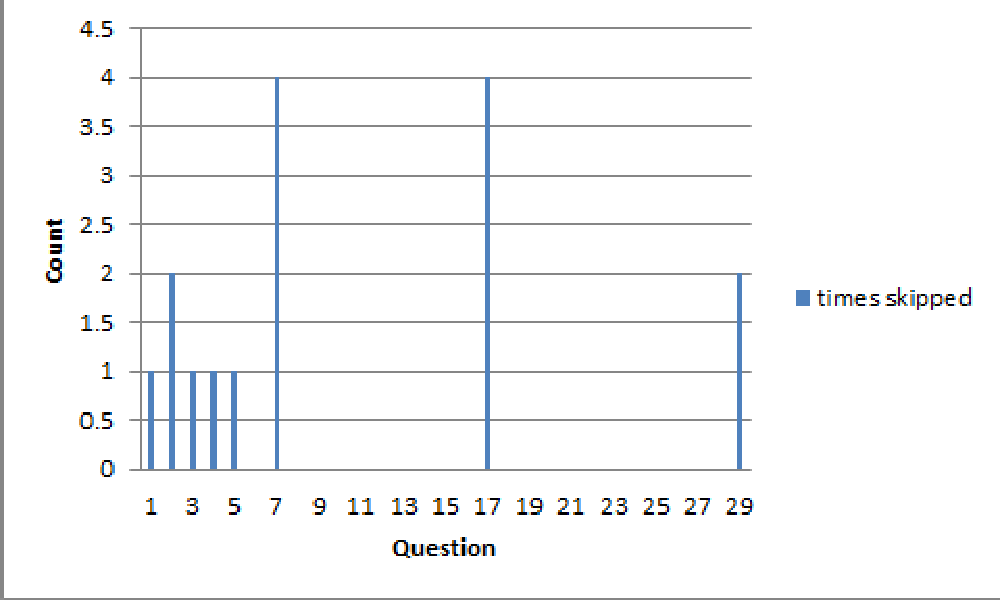
\includegraphics[width=3.01in,height=2.01in]{figure2}
\caption{Caption }
\end{figure}


Question 7 and 17 were skipped 4 times each, these two questions are follow
up questions to questions 6 and 16 and we were trying to collect more
details about user's responses in questions 6 and 16.

\label{sec:appendices}

\end{document}
